\chapter{\ifproject%
\ifenglish Experimentation and Results\else การทดลองและผลลัพธ์\fi
\else%
\ifenglish System Evaluation\else การประเมินระบบ\fi
\fi}

ในบทนี้จะกล่าวที่ผลลัพธ์ของโครงงานเมื่อสร้างเสร็จและฟังก์ชันการทำ หลักๆ จะมีการเทรนบอทให้มี
การตอบที่เป็นธรรมชาติ และมีความแม่นยำถูกต้องในการตอบ ตลอดจนไปถึงความพึงพอใจของผู้ใช้งาน
\section{การประเมินประสิทธิภาพ (Performance evaluation)}
สามารถจำแบบออกเป็น 2 หัวข้อดังนี้
\subsection{ความถูกต้องในการตอบคำถาม (Accuracy)}
โดยจะจัดทำ data set สำหรับการทดสอบและบันทึกผลโดยมีเป้าหมายคือมีความแม่ยำมากกว่า 85\% ขึ้นไป

\begin{figure}[hbt!]
  \begin{center}
    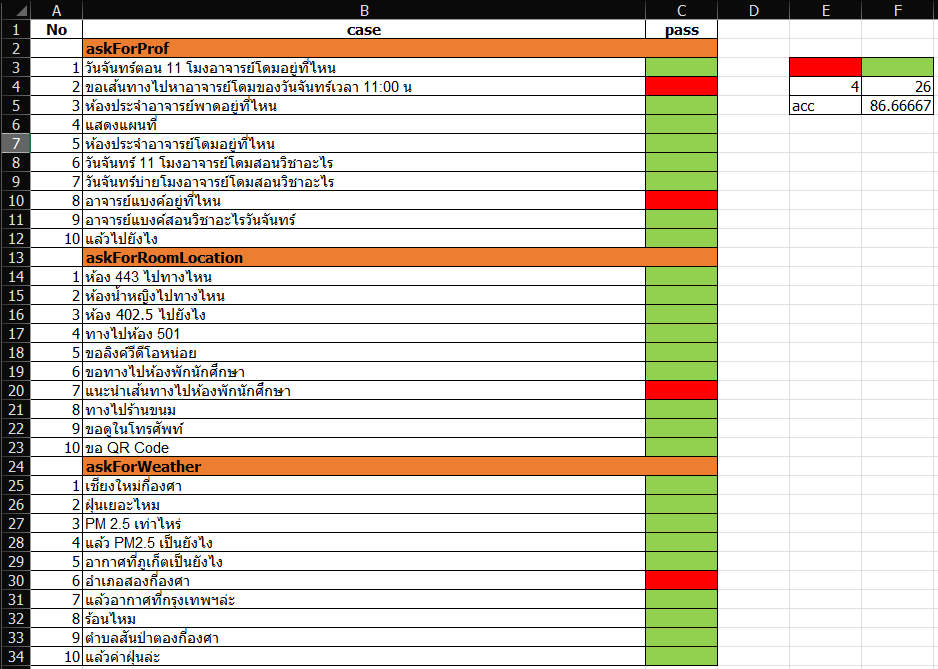
\includegraphics[width=\textwidth,keepaspectratio]{pic/eval_bot_accuracy.png}
  \end{center}
  \caption{ภาพแสดงถึงผลการทดสอบสำหรับประเมินความถูกต้องในการตอบคําถาม}
  \label{fig:eval_bot_accuracy}
\end{figure}

การทดลองพบว่าโครงงานสามารถตอบคำถามได้ถูกต้องมากกว่า 85\% และมีความแม่นยำอยู่ที่ 86.66\% ซึ่งสามารถตอบคำถามได้ดีเพียงพอต่อการใช้งานจริง
แต่ยังคงมีความคลาดเคลื่อนในการตอบคำถามอยู่บ้าง
\subsection{ความรวดเร็วในการทำงาน (Response time)}
โดยจะทำการทดลองส่ง request ไปยังตัว Dialogflow และวัดเวลาในการตอบกลับโดยใช้ Postman ในการดู response time ของ API

\begin{figure}[hbt!]
  \begin{center}
    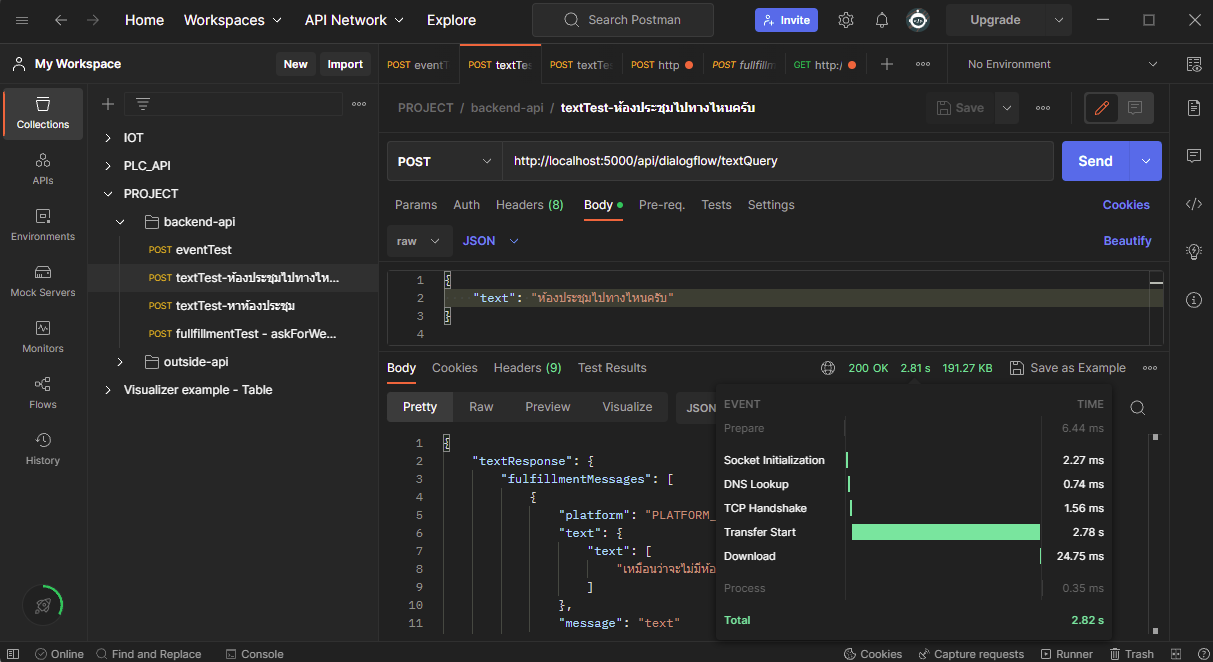
\includegraphics[width=\textwidth,keepaspectratio]{pic/eval_bot_response_time.png}
  \end{center}
  \caption{ภาพแสดงถึงวิธีการทดสอบสำหรับประเมินความรวดเร็วในการทำงานใน postman}
  \label{fig:eval_bot_response_time}
\end{figure}

\begin{figure}[hbt!]
  \begin{center}
    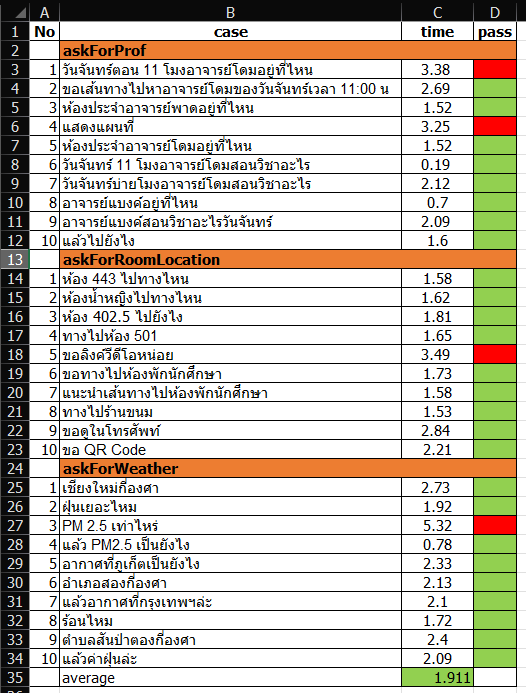
\includegraphics[width=\textwidth,keepaspectratio]{pic/eval_bot_response_time_table.png}
  \end{center}
  \caption{ภาพแสดงถึงผลการทดสอบสำหรับประเมินความรวดเร็วในการทำงาน}
  \label{fig:eval_bot_response_time_table}
\end{figure}

การวัดเวลาการตอบคำถามพบว่าค่าเฉลี่ยของความเร็วในการตอบคำถามน้อยกว่า 3 วินาทีและมีค่าเฉลี่ยอยู่ที่ 1.911 วินาที
ซึ่งอยู่ในเกณฑ์ที่เหมาะสมสำหรับการใช้งานจริง

เพื่อเพิ่มประสิทธิภาพในการตอบคำถามและลดความคลาดเคลื่อนในการตอบคำถาม อาจจะต้องพัฒนาโมเดลแชทบอทเพิ่มเติมเพื่อเพิ่มความถูกต้องในการตอบคำถาม
และต้องปรับปรุงอัลกอริทึมในการดึงข้อมูลจากฐานข้อมูลและ API เพื่อลดเวลาในการตอบคำถามอีกด้วย